\documentclass[border=5pt]{standalone}
\usepackage{tikz}
\usetikzlibrary{positioning, calc, fit, matrix}

\begin{document}

% ============================================================
%  SCENE
% ============================================================
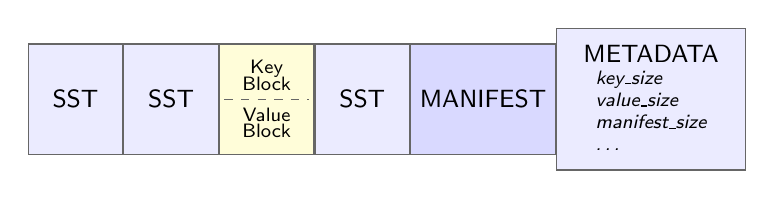
\begin{tikzpicture}[
    % Block styles
    sst/.style={
      rectangle, draw=black!60, fill=blue!8,
      minimum width=1.2cm, minimum height=1cm,
      font=\sffamily\small, align=center
    },
    sst-expanded/.style={
      rectangle, draw=black!60, fill=yellow!15,
      minimum width=1.2cm, minimum height=1cm,
      font=\sffamily\small, align=center
    },
    manifest/.style={
      rectangle, draw=black!60, fill=blue!15,
      minimum width=1.8cm, minimum height=1cm,
      font=\sffamily\small, align=center
    },
    metadata/.style={
      rectangle, draw=black!60, fill=blue!8,
      minimum width=2.4cm,
      font=\sffamily\small, align=center
    },
    logblock/.style={minimum height=1.4cm},
    file/.style={
      draw=black!60, fill=blue!8, rounded corners=2pt,
      minimum width=2.8cm, minimum height=0.7cm,
      font=\ttfamily\scriptsize
    },
    connector/.style={draw=black!50, thick},
  ]

  % === Log Bar (anchor element) ===
  \node[sst, logblock] (sst1) {SST};
  \node[sst, logblock, right=0pt of sst1] (sst2) {SST};

  % Expanded SST
  \node[sst-expanded, logblock, right=0pt of sst2] (sst3) {};
  \draw[dashed, black!60] ([xshift=2pt]sst3.west) -- ([xshift=-2pt]sst3.east);
  \node[font=\sffamily\scriptsize, align=center] at ([yshift=0.3cm]sst3.center) {Key\\[-2pt]Block};
  \node[font=\sffamily\scriptsize, align=center] at ([yshift=-0.3cm]sst3.center) {Value\\[-2pt]Block};

  \node[sst, logblock, right=0pt of sst3] (sst4) {SST};
  \node[manifest, logblock, right=0pt of sst4] (man) {MANIFEST};
  \node[metadata, logblock, right=0pt of man, minimum height=1.8cm] (meta) {};
  \node[font=\sffamily\small, anchor=north] at ([yshift=-0.1cm]meta.north) {METADATA};
  \node[font=\sffamily\scriptsize\itshape, align=left, anchor=center] at ([yshift=-0.15cm]meta.center) {key\_size\\value\_size\\manifest\_size\\\ldots};

  % === COMMENTED OUT FOR NOW ===
  % % === Index Table (above right of log bar) ===
  % \matrix[
  %   matrix of nodes,
  %   above right=0.8cm and -1cm of meta.north east,
  %   anchor=south east,
  %   nodes={font=\sffamily\small, minimum height=0.6cm, anchor=center},
  %   column 1/.style={nodes={minimum width=1.8cm}},
  %   column 2/.style={nodes={minimum width=1.2cm}},
  %   column 3/.style={nodes={minimum width=1.2cm}},
  %   column 4/.style={nodes={minimum width=1.2cm}},
  %   row 1/.style={nodes={fill=blue!15, font=\sffamily\small\bfseries}},
  %   row 2/.style={nodes={fill=yellow!15}},
  %   row 3/.style={nodes={fill=yellow!15}},
  %   row 4/.style={nodes={fill=yellow!15}},
  %   row 5/.style={nodes={fill=yellow!15}},
  % ] (table) {
  %   Log Offset & First & Last & Length \\
  %   0 & 0.031 & 0.036 & 1000 \\
  %   44000 & 0.032 & 0.035 & 832 \\
  %   80608 & 0.03 & 0.038 & 360 \\
  %   96448 & \ldots & \ldots & \ldots \\
  % };
  % \draw[black!60] (table.north west) rectangle (table.south east);

  % % === Keys Callout (left of log bar) ===
  % \node[
  %   draw=black!60, rounded corners=4pt,
  %   fill=white,
  %   font=\sffamily\small,
  %   align=center,
  %   inner sep=6pt,
  %   left=1cm of sst1
  % ] (callout) {0.03, 0.031,\\0.033, \ldots, 0.038};

  % % Connector lines from callout
  % \draw[connector] (callout.north east) -- (table.south west);
  % \draw[connector] (callout.east) -- (sst1.west);

  % % === Stacked Files (below log bar) ===
  % % Left stack
  % \node[file, below=1.2cm of sst1.south, anchor=north, xshift=0.3cm, yshift=-0.3cm] (f2) {koidb.log.rank2};
  % \node[file, below=1.2cm of sst1.south, anchor=north, xshift=0.15cm, yshift=-0.15cm] (f1) {koidb.log.rank1};
  % \node[file, below=1.2cm of sst1.south, anchor=north] (f0) {koidb.log.rank0};

  % % Right stack
  % \node[file, below=1.2cm of meta.south, anchor=north, xshift=0.3cm, yshift=-0.3cm] (f511) {koidb.log.rank511};
  % \node[file, below=1.2cm of meta.south, anchor=north, xshift=0.15cm, yshift=-0.15cm] (f510) {koidb.log.rank510};
  % \node[file, below=1.2cm of meta.south, anchor=north] (f509) {koidb.log.rank509};

  % % Ellipsis
  % \node[font=\sffamily\Large] at ($(f0.east)!0.5!(f509.west)$) {\textbf{\ldots}};

\end{tikzpicture}

\end{document}
